\part{Induction machine}
\title[Induction machine]{Induction machine}  
\date{}  
\frame{\titlepage} 

%%%%%%%%%%%%%%%%%%%%%%%%%%%%%%%%%%%%%%%%%%%%%%%%%%%%%%%%%%%%%
%% Basic induction machine (IM) representation %%
%%%%%%%%%%%%%%%%%%%%%%%%%%%%%%%%%%%%%%%%%%%%%%%%%%%%%%%%%%%%%
\begin{frame}
	\frametitle{Basic induction machine (IM) representation}
    \begin{columns}
		\begin{column}{0.55\textwidth}
	       \begin{itemize}
            \item Three-phase stator + three-phase rotor: ``rotating three-phase transformer''\newline (plus air gap)
            \item Rotor angular speed: $\omega_\mathrm{r}$
            \item Rotor angular displacement: $\varepsilon_\mathrm{r}$
            \item Index ``s'' for stator, ``r'' for rotor quantities
           \end{itemize}
           \begin{varblock}{Fundamental wave model}
              While the previous chapter has revealed that the magnetic flux distribution in the air gap is subject to plentiful harmonics, the following model limits itself to the fundamental wave.
           \end{varblock}
        \end{column}
        \begin{column}{0.45\textwidth}
            \begin{figure}
                \centering
                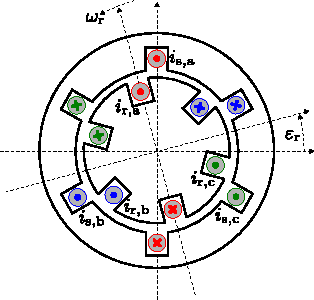
\includegraphics[width=0.85\textwidth]{fig/lec06/Simple_three_phase_induction_machine_lumped_coils.pdf}
                \caption{Elementary three-phase induction machine (IM) lumped-coil representation ($p=1$ pole pair)}
                \label{fig:Simple_three_phase_induction_machine_lumped_coils}
            \end{figure}
        \end{column}
    \end{columns}
\end{frame}

%%%%%%%%%%%%%%%%%%%%%%%%%%%%%%%%%%%%%%%%%%%%%%%%%%%%%%%%%%%%%
%% Dynamical IM model %%
%%%%%%%%%%%%%%%%%%%%%%%%%%%%%%%%%%%%%%%%%%%%%%%%%%%%%%%%%%%%%
\begin{frame}
	\frametitle{Dynamical IM model}
    Based on Faraday's and Ohm's laws, we can write the following equations for the stator 
    \begin{equation}
            \bm{u}^\mathrm{s}_\mathrm{s,abc}(t) = R_\mathrm{s}\bm{i}^\mathrm{s}_\mathrm{s,abc}(t)+\frac{\mathrm{d}}{\mathrm{d}t}\bm{\psi}^\mathrm{s}_\mathrm{s,abc}(t) \hspace{0.2cm} \Leftrightarrow \hspace{0.2cm} \begin{bmatrix}
                u_{\mathrm{s,a}}^\mathrm{s}(t)\\
                u_{\mathrm{s,b}}^\mathrm{s}(t)\\
                u_{\mathrm{s,c}}(t)\\
            \end{bmatrix} = R_\mathrm{s} \begin{bmatrix}
                i_{\mathrm{s,a}}^\mathrm{s}(t)\\
                i_{\mathrm{s,b}}^\mathrm{s}(t)\\
                i_{\mathrm{s,c}}^\mathrm{s}(t)\\
            \end{bmatrix} + \frac{\mathrm{d}}{\mathrm{d}t} \begin{bmatrix}
                \psi_{\mathrm{s,a}}^\mathrm{s}(t)\\
                \psi_{\mathrm{s,b}}^\mathrm{s}(t)\\
                \psi_{\mathrm{s,c}}^\mathrm{s}(t)\\
            \end{bmatrix}
            \label{eq:IM_stator_three_phase_voltage_equation}
    \end{equation}
    and rotor
    \begin{equation}
            \bm{u}^\mathrm{r}_\mathrm{r,abc}(t) = R_\mathrm{r}\bm{i}^\mathrm{r}_\mathrm{r,abc}(t)+\frac{\mathrm{d}}{\mathrm{d}t}\bm{\psi}^\mathrm{r}_\mathrm{r,abc}(t) \hspace{0.2cm} \Leftrightarrow \hspace{0.2cm} \begin{bmatrix}
                u_{\mathrm{r,a}}^\mathrm{r}(t)\\
                u_{\mathrm{r,b}}^\mathrm{r}(t)\\
                u_{\mathrm{r,c}}^\mathrm{r}(t)\\
            \end{bmatrix} = R_\mathrm{r} \begin{bmatrix}
                i_{\mathrm{r,a}}^\mathrm{r}(t)\\
                i_{\mathrm{r,b}}^\mathrm{r}(t)\\
                i_{\mathrm{r,c}}^\mathrm{r}(t)\\
            \end{bmatrix} + \frac{\mathrm{d}}{\mathrm{d}t} \begin{bmatrix}
                \psi_{\mathrm{r,a}}^\mathrm{r}(t)\\
                \psi_{\mathrm{r,b}}^\mathrm{r}(t)\\
                \psi_{\mathrm{r,c}}^\mathrm{r}(t)\\
            \end{bmatrix}
            \label{eq:IM_rotor_three_phase_voltage_equation}
    \end{equation}
which are generally applicable as only identical resistances per phase on the stator and rotor are assumed. Above, the lower index denotes the physical location of the quantities, while the upper index indicates the coordinate system orientation.
\end{frame}

%%%%%%%%%%%%%%%%%%%%%%%%%%%%%%%%%%%%%%%%%%%%%%%%%%%%%%%%%%%%%
%% Flux linakge model %%
%%%%%%%%%%%%%%%%%%%%%%%%%%%%%%%%%%%%%%%%%%%%%%%%%%%%%%%%%%%%%
\begin{frame}
	\frametitle{Flux linkage model}
    \begin{columns}
		\begin{column}{0.55\textwidth}
            In contrast to the simple three-phase transformer model \eqref{eq:Three_phase_transformer_flux_linkage}, the flux linkage model of the IM is more complex: 
	       \begin{itemize}
            \item Due to the spatial 120$^\circ$ phase shift between the windings of the stator and rotor, the abc phases are all mutually coupled.
            \item The flux paths and physical dimensions of the stator and rotor are not identical, i.e., the rotor and stator inductances are different (even if the winding turns $N_\mathrm{s}$ and $N_\mathrm{r}$ are identical).
            \item The coupling between the stator and rotor is rotor position-dependent (not explicitly shown on the right due to space limitations). 
           \end{itemize}
        \end{column}
        \begin{column}{0.45\textwidth}
            \begin{figure}
                \centering
                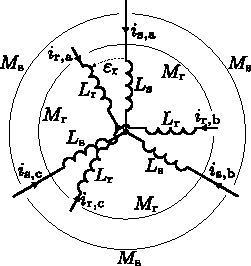
\includegraphics[width=0.75\textwidth]{fig/lec06/Inductive_coupling_stator_rotor.pdf}
                \caption{Simplified representation of the inductive coupling between the stator/rotor phases}
                \label{fig:Simple_three_phase_induction_machine_lumped_coils}
            \end{figure}
        \end{column}
    \end{columns}
\end{frame}

%%%%%%%%%%%%%%%%%%%%%%%%%%%%%%%%%%%%%%%%%%%%%%%%%%%%%%%%%%%%%
%% Flux linakge model %%
%%%%%%%%%%%%%%%%%%%%%%%%%%%%%%%%%%%%%%%%%%%%%%%%%%%%%%%%%%%%%
\begin{frame}
	\frametitle{Flux linkages of the three-phase model}
    Based on the previous considerations, the flux linkages are given by
    \begin{equation}
        \renewcommand*{\arraystretch}{1.15}
        \begin{split}
            \bm{\psi}^\mathrm{s}_\mathrm{s,abc}(t) &=\begin{bmatrix}
                L_\mathrm{s} & -\frac{M_\mathrm{s}}{2} & -\frac{M_\mathrm{s}}{2}\\
                -\frac{M_\mathrm{s}}{2} & L_\mathrm{s} & -\frac{M_\mathrm{s}}{2}\\
                -\frac{M_\mathrm{s}}{2} & -\frac{M_\mathrm{s}}{2} & L_\mathrm{s}
            \end{bmatrix} \bm{i}^\mathrm{s}_\mathrm{s,abc}(t) +  M_{\mathrm{r}}\frac{N_\mathrm{s}}{N_\mathrm{r}} \bm{\mathcal{R}}_\mathrm{abc}(\varepsilon_\mathrm{r,el}(t))\bm{i}^\mathrm{r}_\mathrm{r,abc}(t),\\
            \bm{\psi}^\mathrm{r}_\mathrm{r,abc}(t) &= \begin{bmatrix}
                L_\mathrm{r} & -\frac{M_\mathrm{r}}{2} & -\frac{M_\mathrm{r}}{2}\\
                -\frac{M_\mathrm{r}}{2} & L_\mathrm{r} & -\frac{M_\mathrm{r}}{2}\\
                -\frac{M_\mathrm{r}}{2} & -\frac{M_\mathrm{r}}{2} & L_\mathrm{r}
            \end{bmatrix} \bm{i}^\mathrm{r}_\mathrm{r,abc}(t) +  M_{\mathrm{s}}\frac{N_\mathrm{r}}{N_\mathrm{s}} \bm{\mathcal{R}}_\mathrm{abc}(\varepsilon_\mathrm{r,el}(t))\T\bm{i}^\mathrm{s}_\mathrm{s,abc}(t) 
        \end{split}
        \label{eq:Flux_linkage_model_IM_abc}
    \end{equation}
    with $\varepsilon_\mathrm{r,el}(t)=p\varepsilon_\mathrm{r}(t)$ and the transformation matrix
    \begin{equation}
        \renewcommand*{\arraystretch}{1.15}
        \bm{\mathcal{R}}_\mathrm{abc}(\varepsilon_\mathrm{r,el}(t)) =\begin{bmatrix}
           \cos(\varepsilon_\mathrm{r,el}(t))  & \cos(\varepsilon_\mathrm{r,el}(t) + \frac{2\pi}{3}) & \cos(\varepsilon_\mathrm{r,el}(t) - \frac{2\pi}{3})\\
            \cos(\varepsilon_\mathrm{r,el}(t) - \frac{2\pi}{3}) & \cos(\varepsilon_\mathrm{r,el}(t)) & \cos(\varepsilon_\mathrm{r,el}(t) + \frac{2\pi}{3})\\
            \cos(\varepsilon_\mathrm{r,el}(t) + \frac{2\pi}{3}) & \cos(\varepsilon_\mathrm{r,el}(t) - \frac{2\pi}{3}) & \cos(\varepsilon_\mathrm{r,el}(t))
        \end{bmatrix}.
    \end{equation}
\end{frame}

%%%%%%%%%%%%%%%%%%%%%%%%%%%%%%%%%%%%%%%%%%%%%%%%%%%%%%%%%%%%%
%% \frametitle{Inductance matrices} %%
%%%%%%%%%%%%%%%%%%%%%%%%%%%%%%%%%%%%%%%%%%%%%%%%%%%%%%%%%%%%%
\begin{frame}
	\frametitle{Inductance matrices of the three-phase model}
    The inductance matrices
    $$\renewcommand*{\arraystretch}{1.15} 
    \bm{L}_\mathrm{s,abc} = \begin{bmatrix}
        L_\mathrm{s} & -\frac{M_\mathrm{s}}{2} & -\frac{M_\mathrm{s}}{2}\\
        -\frac{M_\mathrm{s}}{2} & L_\mathrm{s} & -\frac{M_\mathrm{s}}{2}\\
        -\frac{M_\mathrm{s}}{2} & -\frac{M_\mathrm{s}}{2} & L_\mathrm{s}
    \end{bmatrix}, \qquad  \bm{L}_\mathrm{r,abc} = \begin{bmatrix}
        L_\mathrm{r} & -\frac{M_\mathrm{r}}{2} & -\frac{M_\mathrm{r}}{2}\\
        -\frac{M_\mathrm{r}}{2} & L_\mathrm{r} & -\frac{M_\mathrm{r}}{2}\\
        -\frac{M_\mathrm{r}}{2} & -\frac{M_\mathrm{r}}{2} & L_\mathrm{r}
    \end{bmatrix}$$
    are based on the following considerations. 
    \begin{itemize}
        \item The self-inductances cover both the leakage and mutual coupling to other windings: $L_\mathrm{s/r}=L_\mathrm{s/r, \sigma} + M_\mathrm{s/r}$.
        \item The mutual inductances on the stator/rotor $M_\mathrm{s/r}$ are identical, as all three phases share the same magnetic paths and have the same winding turns $N_\mathrm{s/r}$.
        \item The mutual inductances on the off diagonal represent the spatial displacement of the stator/rotor coils by $\pm 120^\circ$, which is why they are multiplied by $\cos(\pm 120^\circ)=-0.5$.
        \item In \eqref{eq:Flux_linkage_model_IM_abc}, the coupling term between stator and rotor is multiplied by the turn ratio to account for the different winding turns $N_\mathrm{s/r}$ (i.e., mapping the mutual inductances between stator/rotor).
    \end{itemize}
\end{frame}

%%%%%%%%%%%%%%%%%%%%%%%%%%%%%%%%%%%%%%%%%%%%%%%%%%%%%%%%%%%%%
%% Orthogonal representation: alpha-beta coordinates %%
%%%%%%%%%%%%%%%%%%%%%%%%%%%%%%%%%%%%%%%%%%%%%%%%%%%%%%%%%%%%%
\begin{frame}
	\frametitle{Orthogonal representation: alpha-beta coordinates}
    \begin{columns}
		\begin{column}{0.55\textwidth}
	       \begin{itemize}
            \item The three-phase IM model is obviously quite unhandy: six differential equations plus a rather complicated magnetic circuit representation.
            \item Remedy: transform the three-phase model into the orthogonal $\alpha\beta$ coordinates.
            \item Advantage: only four differential equations and a simpler magnetic circuit representation (as one will see on the next slides).
           \end{itemize}
           \vspace{-0.4cm}
           \begin{varblock}{Coordinate transformations}
              The following transformations of the IM model into different coordinate systems are pure mathematical ``tricks'' to simplify the analysis. The IM remains a three-phase machine. 
           \end{varblock}
        \end{column}
        \begin{column}{0.45\textwidth}
            \begin{figure}
                \centering
                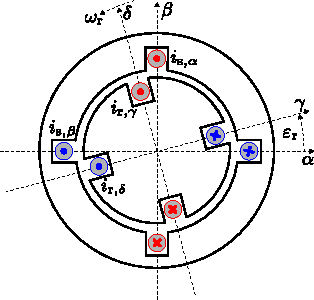
\includegraphics[width=0.85\textwidth]{fig/lec06/Induction_machine_alpha_beta.pdf}
                \caption{Conceptual IM representation within the orthogonal $\alpha\beta$ coordinates ($p=1$ pole pair)}
                \label{fig:Induction_machine_alpha_beta}
            \end{figure}
        \end{column}
    \end{columns}
\end{frame}

%%%%%%%%%%%%%%%%%%%%%%%%%%%%%%%%%%%%%%%%%%%%%%%%%%%%%%%%%%%%%
%% Clarke transformation %%
%%%%%%%%%%%%%%%%%%%%%%%%%%%%%%%%%%%%%%%%%%%%%%%%%%%%%%%%%%%%%
\begin{frame}
	\frametitle{Clarke transformation}
    To transform the three-phase model into the orthogonal $\alpha\beta$ coordinates, the Clarke transformation is applied. Consider any $\bm{x}_\mathrm{abc}\in\mathbb{R}^3$, then the Clarke transformation is given by
    \begin{equation}
        \renewcommand{\arraystretch}{1.2}
        \bm{x}_{\alpha \beta0} = \begin{bmatrix} x_\alpha \\ x_\beta \\ x_0\end{bmatrix} = \begin{bmatrix}
            \nicefrac{2}{3} & -\nicefrac{1}{3} & -\nicefrac{1}{3}\\
            0 & \nicefrac{1}{\sqrt{3}} & -\nicefrac{1}{\sqrt{3}}\\
            \nicefrac{\sqrt{2}}{3} & \nicefrac{\sqrt{2}}{3} & \nicefrac{\sqrt{2}}{3}
        \end{bmatrix} \begin{bmatrix} x_\mathrm{a} \\ x_\mathrm{b} \\ x_\mathrm{c}\end{bmatrix} = \bm{T}_\mathrm{c} \bm{x}_\mathrm{abc} 
        \label{eq:Clarke_transformation}
    \end{equation}
    with the inverse transformation
    \begin{equation}
        \renewcommand{\arraystretch}{1.2}
        \bm{x}_\mathrm{abc}  = \begin{bmatrix}
            1 & 0 & \nicefrac{1}{\sqrt{2}}\\
            -\nicefrac{1}{2} & \nicefrac{\sqrt{3}}{2} & \nicefrac{1}{\sqrt{2}}\\
            -\nicefrac{1}{2} & -\nicefrac{\sqrt{3}}{2} & \nicefrac{1}{\sqrt{2}}
        \end{bmatrix} \begin{bmatrix} x_\alpha \\ x_\beta \\ x_0\end{bmatrix} = \bm{T}_\mathrm{c}^{-1} \bm{x}_{\alpha \beta 0}.
    \end{equation}
    Above, $\bm{T}_\mathrm{c}\in\mathbb{R}^{3\times 3}$ is the Clarke transformation matrix and $\bm{x}_\mathrm{\alpha \beta0}\in\mathbb{R}^3$ the transformed vector.
\end{frame}

%%%%%%%%%%%%%%%%%%%%%%%%%%%%%%%%%%%%%%%%%%%%%%%%%%%%%%%%%%%%%
%% Clarke transformation: amplitude and power scaling %%
%%%%%%%%%%%%%%%%%%%%%%%%%%%%%%%%%%%%%%%%%%%%%%%%%%%%%%%%%%%%%
\begin{frame}
	\frametitle{Clarke transformation: amplitude and power scaling}
    The transformation \eqref{eq:Clarke_transformation} is amplitude-preserving, i.e., the amplitude of the $\alpha\beta$ vector is identical to the amplitude of the original abc vector. On the other hand, the power is not preserved, as can be seen from the inner product of the transformed vectors (which commonly occurs in power calculations):
    \begin{equation*}
        \bm{x}_{\mathrm{abc}}\T \bm{y}_{\mathrm{abc}} = \bm{x}_\mathrm{\alpha \beta 0}\T\left(\bm{T}_\mathrm{c}^{-1}\right)\T \bm{T}_\mathrm{c}^{-1}\bm{y}_\mathrm{\alpha \beta 0} \quad \Leftrightarrow \quad x_\mathrm{a}y_\mathrm{a} + x_\mathrm{b}y_\mathrm{b} + x_\mathrm{c}y_\mathrm{c} = \frac{3}{2}\left(x_\alpha y_\alpha + x_\beta y_\beta + x_0 y_0 \right).
    \end{equation*}
    The alternative power-preserving Clarke transformation variant is given by
    \begin{equation}
        \renewcommand{\arraystretch}{1.2}
        \bm{T}'_\mathrm{c} = \frac{\sqrt{3}}{2} \bm{T}_\mathrm{c} \qquad \left(\bm{T}'_\mathrm{c}\right)^{-1} = \left(\bm{T}'_\mathrm{c}\right)\T,
        \label{eq:Clarke_transformation_power_preserving}
    \end{equation}
    which utilizes an orthogonal transformation matrix. However, when using $\bm{T}'_\mathrm{c}$ the amplitude of the transformed vector is not preserved. While being an arbitrary choice, we will stick to \eqref{eq:Clarke_transformation} as a convention for the following. 
\end{frame}

%%%%%%%%%%%%%%%%%%%%%%%%%%%%%%%%%%%%%%%%%%%%%%%%%%%%%%%%%%%%%
%% Clarke transformation: simplification for zero-component-free vectors %%
%%%%%%%%%%%%%%%%%%%%%%%%%%%%%%%%%%%%%%%%%%%%%%%%%%%%%%%%%%%%%
\begin{frame}
	\frametitle{Clarke transformation: simplification for zero-component-free vectors}
    If the abc vector $\bm{x}_\mathrm{abc}$ is zero-component-free, i.e.,  $$x_\mathrm{a} + x_\mathrm{b} +x_\mathrm{c} = 0,$$
    e.g., the phase currents of a star connected system, the Clarke transformation simplifies to
    \begin{equation}
        \renewcommand{\arraystretch}{1.2}
        \bm{x}_{\alpha \beta} = \begin{bmatrix} x_\alpha \\ x_\beta \end{bmatrix} = \begin{bmatrix}
            \nicefrac{2}{3} & -\nicefrac{1}{3} & -\nicefrac{1}{3}\\
            0 & \nicefrac{1}{\sqrt{3}} & -\nicefrac{1}{\sqrt{3}}
        \end{bmatrix} \begin{bmatrix} x_\mathrm{a} \\ x_\mathrm{b} \\ x_\mathrm{c}\end{bmatrix} = \bm{T}_{23} \bm{x}_\mathrm{abc}
        \label{eq:Clarke_transformation_zero_component_free}
    \end{equation}
    and
    \begin{equation}
        \renewcommand{\arraystretch}{1.2}
        \bm{x}_\mathrm{abc}  = \begin{bmatrix}
            1 & 0\\
            -\nicefrac{1}{2} & \nicefrac{\sqrt{3}}{2}\\
            -\nicefrac{1}{2} & -\nicefrac{\sqrt{3}}{2}
        \end{bmatrix} \begin{bmatrix} x_\alpha \\ x_\beta \end{bmatrix} = \bm{T}_{32} \bm{x}_{\alpha \beta}.
    \end{equation}     
\end{frame}

%%%%%%%%%%%%%%%%%%%%%%%%%%%%%%%%%%%%%%%%%%%%%%%%%%%%%%%%%%%%%
%% Clarke transformation: simplification for zero-component-free vectors %%
%%%%%%%%%%%%%%%%%%%%%%%%%%%%%%%%%%%%%%%%%%%%%%%%%%%%%%%%%%%%%
\begin{frame}
	\frametitle{Clarke transformation: simplification for zero-component-free vectors}
    \begin{figure}
        \centering
        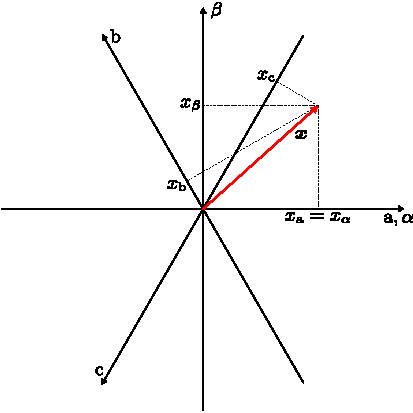
\includegraphics[width=0.38\textwidth]{fig/lec06/abc_alphabeta_vectors.pdf}
        \caption{Geometrical interpretation of the Clarke
        transformation without zero components: mapping $\bm{x}_\mathrm{abc}\in\mathbb{R}^3$ to $\bm{x}_{\alpha\beta}\in\mathbb{R}^2$ without information loss (adapted from J.~B\"ocker, \textit{Controlled Three-Phase Drives}, Paderborn University, 2021)}
        \label{fig:abc_alphabeta_vectors}
    \end{figure}    
\end{frame}


%%%%%%%%%%%%%%%%%%%%%%%%%%%%%%%%%%%%%%%%%%%%%%%%%%%%%%%%%%%%%
%% Park transformation %%
%%%%%%%%%%%%%%%%%%%%%%%%%%%%%%%%%%%%%%%%%%%%%%%%%%%%%%%%%%%%%
\begin{frame}
	\frametitle{Park transformation}
    The Park transform rotates a vector $\bm{x}_{\alpha \beta}\in\mathbb{R}^2$ by a certain angle $\varepsilon$ to obtain $\bm{x}_\mathrm{dq}\in\mathbb{R}^2$, that is, 
    \begin{equation}
        \renewcommand{\arraystretch}{1.2}
        \bm{x}_{\mathrm{dq}} = \begin{bmatrix} x_\mathrm{d} \\ x_\mathrm{q} \end{bmatrix} = \begin{bmatrix}
            \cos(\varepsilon) & \sin(\varepsilon)\\
            -\sin(\varepsilon) & \cos(\varepsilon)
        \end{bmatrix} \begin{bmatrix} x_\alpha \\ x_\beta \end{bmatrix} = \bm{T}_\mathrm{p}^{-1} \bm{x}_\mathrm{\alpha \beta} 
        \label{eq:Park_transformation}
    \end{equation}
    with the counter rotation
    \begin{equation}
        \renewcommand{\arraystretch}{1.2}
        \bm{x}_{\alpha \beta} = \begin{bmatrix}
            \cos(\varepsilon) & -\sin(\varepsilon)\\
            \sin(\varepsilon) & \cos(\varepsilon)
        \end{bmatrix} \begin{bmatrix} x_\mathrm{d} \\ x_\mathrm{q} \end{bmatrix} = \bm{T}_\mathrm{p} \bm{x}_{\mathrm{dq}}.
    \end{equation}
    Above, $\bm{T}_\mathrm{p}\in\mathbb{R}^{2\times 2}$ is the Park transformation matrix. It might be noted that is a (historical) convention to define that $\bm{T}_\mathrm{p}$ rotates into the mathematically positive direction. Depending on the application background and choice of $\varepsilon$, the interpretation of $\bm{x}_\mathrm{dq}$ can vary.
\end{frame}

%%%%%%%%%%%%%%%%%%%%%%%%%%%%%%%%%%%%%%%%%%%%%%%%%%%%%%%%%%%%%
%% Park transformation (cont.) %%
%%%%%%%%%%%%%%%%%%%%%%%%%%%%%%%%%%%%%%%%%%%%%%%%%%%%%%%%%%%%%
\begin{frame}
	\frametitle{Park transformation (cont.)}
    \begin{figure}
        \centering
        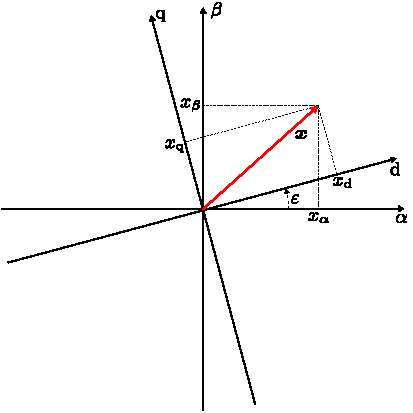
\includegraphics[width=0.4\textwidth]{fig/lec06/Alphabeta_dq_vectors.pdf}
        \caption{Geometrical interpretation of the Park
        transformation: mapping $\bm{x}_{\alpha\beta}\in\mathbb{R}^2$ to $\bm{x}_{\mathrm{dq}}\in\mathbb{R}^2$ (adapted from J.~B\"ocker, \textit{Controlled Three-Phase Drives}, Paderborn University, 2021)}
        \label{fig:Alphabeta_dq_vectors}
    \end{figure}    
\end{frame}

%%%%%%%%%%%%%%%%%%%%%%%%%%%%%%%%%%%%%%%%%%%%%%%%%%%%%%%%%%%%%
%% Park transformation: some properties %%
%%%%%%%%%%%%%%%%%%%%%%%%%%%%%%%%%%%%%%%%%%%%%%%%%%%%%%%%%%%%%
\begin{frame}
	\frametitle{Park transformation: some properties}
    Performing the Park and inverse Park transformation sequentially, does not change the vector:
    \begin{equation}
        \bm{x}_{\alpha \beta} = \bm{T}_\mathrm{p} \bm{T}_\mathrm{p}^{-1} \bm{x}_{\alpha \beta} = \bm{T}_\mathrm{p}^{-1} \bm{T}_\mathrm{p} \bm{x}_{\alpha \beta}.
    \end{equation}
    A frequent rotation within the electric machines and drives context is
    \begin{equation}
        \renewcommand{\arraystretch}{1.1}
         \bm{T}_\mathrm{p}(\varepsilon = \nicefrac{\pi}{2}) = \begin{bmatrix}
            \cos(\nicefrac{\pi}{2}) & -\sin(\nicefrac{\pi}{2})\\
            \sin(\nicefrac{\pi}{2}) & \cos(\nicefrac{\pi}{2})
        \end{bmatrix} = \begin{bmatrix}
            0 & -1\\
            1 & 0
        \end{bmatrix} = \bm{J}
    \end{equation}
    leading to the definition of $\bm{J}\in\mathbb{R}^{2 \times 2}$ which will be used for brevity in the following.  Moreover, if $\varepsilon$ results from some rotation, i.e., $\nicefrac{\mathrm{d}}{\mathrm{d}t}\,\varepsilon(t)=\omega(t)$, we have:
    \begin{align}
        \renewcommand{\arraystretch}{1.1}
        \frac{\mathrm{d}}{\mathrm{d}t}\bm{T}_\mathrm{p}(\varepsilon(t)) &= \begin{bmatrix}
            -\sin(\varepsilon(t)) & -\cos(\varepsilon(t))\\
            \cos(\varepsilon(t)) & -\sin(\varepsilon(t))
        \end{bmatrix} \frac{\mathrm{d}}{\mathrm{d}t}\varepsilon(t)  = \bm{T}_\mathrm{p}(\varepsilon(t)) \bm{J}\omega(t),\\
        \frac{\mathrm{d}}{\mathrm{d}t}\bm{T}_\mathrm{p}^{-1}(\varepsilon(t)) &= \begin{bmatrix}
            -\sin(\varepsilon(t)) & \cos(\varepsilon(t))\\
            -\cos(\varepsilon(t)) & -\sin(\varepsilon(t))
        \end{bmatrix} \frac{\mathrm{d}}{\mathrm{d}t}\varepsilon(t)  = -\bm{T}_\mathrm{p}^{-1}(\varepsilon(t)) \bm{J}\omega(t).
    \end{align}
\end{frame}

%%%%%%%%%%%%%%%%%%%%%%%%%%%%%%%%%%%%%%%%%%%%%%%%%%%%%%%%%%%%%
%% Visualization of different coordinate systems %%
%%%%%%%%%%%%%%%%%%%%%%%%%%%%%%%%%%%%%%%%%%%%%%%%%%%%%%%%%%%%%
\begin{frame}
	\frametitle{Visualization of different coordinate systems}
    \begin{figure}
        \centering
        \movie{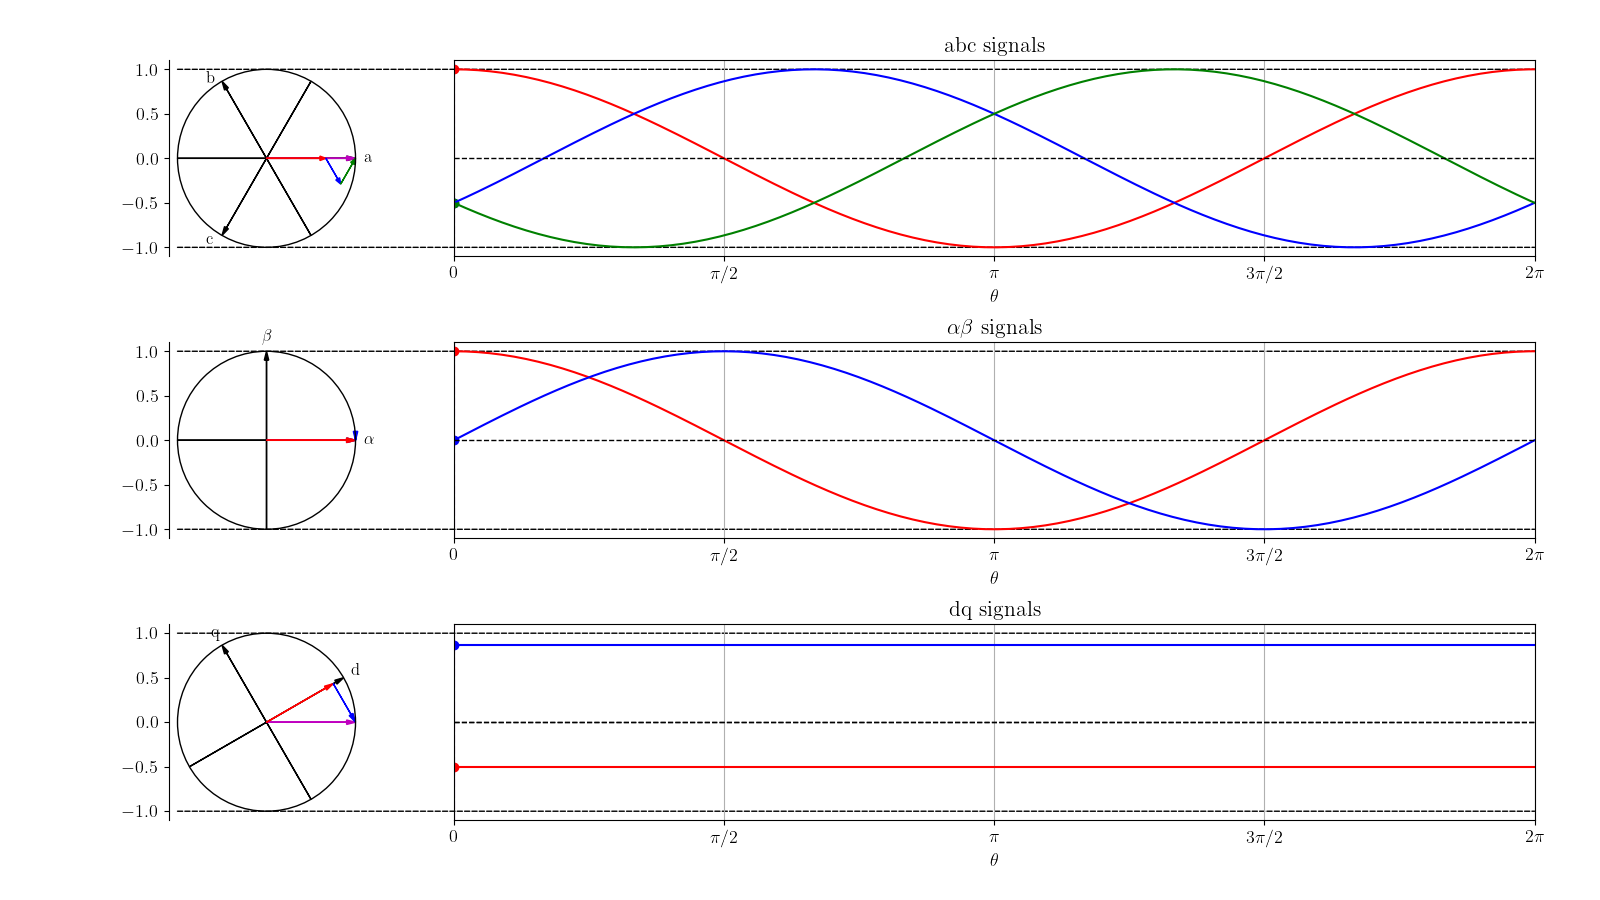
\includegraphics[height=0.8\textheight]{fig/lec06/Clarke_Park_preview.png}}{fig/lec06/Clarke_Park.gif}
        \vspace{-0.25cm}
        \caption{Representation of a rotating phasor (without zero component) in different coordinate systems}
        \label{fig:Clarke_Park_animation}
    \end{figure}
\end{frame}

%%%%%%%%%%%%%%%%%%%%%%%%%%%%%%%%%%%%%%%%%%%%%%%%%%%%%%%%%%%%%
%% IM model $\alpha\beta-\gamma\delta$ coordinates %%
%%%%%%%%%%%%%%%%%%%%%%%%%%%%%%%%%%%%%%%%%%%%%%%%%%%%%%%%%%%%%
\begin{frame}
	\frametitle{IM model $\alpha\beta$ coordinates}
    Assuming zero-component-free three-phase quantities, multiplying the three-phase IM model \eqref{eq:IM_stator_three_phase_voltage_equation} and \eqref{eq:IM_rotor_three_phase_voltage_equation} with $\bm{T}_{23}$ results in
    \begin{equation}
        \begin{split}
        \bm{T}_{23}\bm{u}^\mathrm{s}_\mathrm{s,abc}(t) &= R_\mathrm{s} \bm{T}_{23}\bm{i}^\mathrm{s}_\mathrm{s,abc}(t)+ \bm{T}_{23}\frac{\mathrm{d}}{\mathrm{d}t}\bm{\psi}^\mathrm{s}_\mathrm{s,abc}(t)\\
        \Leftrightarrow\quad \bm{u}^\mathrm{s}_\mathrm{s,\alpha\beta}(t) &= R_\mathrm{s} \bm{i}^\mathrm{s}_\mathrm{s,\alpha\beta}(t)+ \frac{\mathrm{d}}{\mathrm{d}t}\bm{\psi}^\mathrm{s}_\mathrm{s,\alpha\beta}(t) 
    \end{split}
\end{equation}
and
\begin{equation}
    \begin{split}
    \bm{T}_{23}\bm{u}^\mathrm{r}_\mathrm{r,abc}(t) &= R_\mathrm{r} \bm{T}_{23}\bm{i}^\mathrm{r}_\mathrm{r,abc}(t)+ \bm{T}_{23}\frac{\mathrm{d}}{\mathrm{d}t}\bm{\psi}^\mathrm{r}_\mathrm{r,abc}(t)\\
    \Leftrightarrow\quad  \bm{u}^\mathrm{r}_\mathrm{r,\alpha\beta}(t) &= R_\mathrm{r} \bm{i}^\mathrm{r}_\mathrm{r,\alpha\beta}(t)+ \frac{\mathrm{d}}{\mathrm{d}t}\bm{\psi}^\mathrm{r}_\mathrm{r,\alpha\beta}(t).
\end{split}
\end{equation}
Here, it must be noted that the two voltage equations are still represented in their own stator or rotor coordinate system. In particular, the rotor's $\alpha\beta$ axes are rotating (compare \figref{fig:Induction_machine_alpha_beta}). 
\end{frame}

%%%%%%%%%%%%%%%%%%%%%%%%%%%%%%%%%%%%%%%%%%%%%%%%%%%%%%%%%%%%%
%% IM model $\alpha\beta-\gamma\delta$ coordinates %%
%%%%%%%%%%%%%%%%%%%%%%%%%%%%%%%%%%%%%%%%%%%%%%%%%%%%%%%%%%%%%
\begin{frame}
	\frametitle{IM model $\alpha\beta$ coordinates: transformation of rotor quantities}
    To bring both model parts into the same coordinate system, the rotor quantities will be transformed into the stator's $\alpha\beta$ coordinates. This is done by applying the Park transformation with $\varepsilon(t) = \varepsilon_\mathrm{r,el}(t)=p\varepsilon_\mathrm{r}(t)$: 
    \begin{equation}
        \begin{split}
        T_\mathrm{p}(\varepsilon_\mathrm{r,el}(t))\bm{u}^\mathrm{r}_\mathrm{r,\alpha\beta}(t) &= T_\mathrm{p}(\varepsilon_\mathrm{r,el}(t))R_\mathrm{r} \bm{i}^\mathrm{r}_\mathrm{r,\alpha\beta}(t)+ T_\mathrm{p}(\varepsilon_\mathrm{r,el}(t))\frac{\mathrm{d}}{\mathrm{d}t}\bm{\psi}^\mathrm{r}_\mathrm{r,\alpha\beta}(t)\\
        \Leftrightarrow\quad  \bm{u}^\mathrm{s}_\mathrm{r,\alpha\beta}(t)   &= R_\mathrm{r} \bm{i}^\mathrm{s}_\mathrm{r,\alpha\beta}(t)+ T_\mathrm{p}(\varepsilon_\mathrm{r,el}(t))\frac{\mathrm{d}}{\mathrm{d}t}\bm{\psi}^\mathrm{r}_\mathrm{r,\alpha\beta}(t).
        \label{eq:IM_rotor_alpha_beta_voltage_equation_coord_transf_intermediate}
    \end{split}
    \end{equation}
    The last term of \eqref{eq:IM_rotor_alpha_beta_voltage_equation_coord_transf_intermediate} is rewritten as
    \begin{align*}
        T_\mathrm{p}(\varepsilon_\mathrm{r,el}(t))\frac{\mathrm{d}}{\mathrm{d}t}\bm{\psi}^\mathrm{r}_\mathrm{r,\alpha\beta}(t) &= T_\mathrm{p}(\varepsilon_\mathrm{r,el}(t))\frac{\mathrm{d}}{\mathrm{d}t}\left[T_\mathrm{p}^{-1}(\varepsilon_\mathrm{r,el}(t))\bm{\psi}^\mathrm{s}_\mathrm{r,\alpha\beta}(t)\right] \\ &=  T_\mathrm{p}(\varepsilon_\mathrm{r,el}(t))\left[\frac{\mathrm{d}}{\mathrm{d}t}\left(T_\mathrm{p}^{-1}(\varepsilon_\mathrm{r,el}(t))\right)\bm{\psi}^\mathrm{s}_\mathrm{r,\alpha\beta}(t) + T_\mathrm{p}^{-1}(\varepsilon_\mathrm{r,el}(t)) \frac{\mathrm{d}}{\mathrm{d}t}\left(\bm{\psi}^\mathrm{s}_\mathrm{r,\alpha\beta}(t)\right)\right]
        \\ &= -\omega_\mathrm{r,el}(t)\bm{J}\bm{\psi}^\mathrm{s}_\mathrm{r,\alpha\beta}(t) +\frac{\mathrm{d}}{\mathrm{d}t}\bm{\psi}^\mathrm{s}_\mathrm{r,\alpha\beta}(t).
    \end{align*}
\end{frame}

%%%%%%%%%%%%%%%%%%%%%%%%%%%%%%%%%%%%%%%%%%%%%%%%%%%%%%%%%%%%%
%% IM model $\alpha\beta-\gamma\delta$ coordinates (cont.)%%
%%%%%%%%%%%%%%%%%%%%%%%%%%%%%%%%%%%%%%%%%%%%%%%%%%%%%%%%%%%%%
\begin{frame}
	\frametitle{IM model $\alpha\beta$ coordinates: transformation of rotor quantities (cont.)}
    Hence, the IM model voltage equations in the stator-oriented $\alpha\beta$ coordinates are
    \begin{equation}
        \begin{split}
        \bm{u}^\mathrm{s}_\mathrm{s,\alpha\beta}(t) &= R_\mathrm{s} \bm{i}^\mathrm{s}_\mathrm{s,\alpha\beta}(t)+ \frac{\mathrm{d}}{\mathrm{d}t}\bm{\psi}^\mathrm{s}_\mathrm{s,\alpha\beta}(t),\\
        \bm{u}^\mathrm{s}_\mathrm{r,\alpha\beta}(t) &= R_\mathrm{r} \bm{i}^\mathrm{s}_\mathrm{r,\alpha\beta}(t)-\omega_\mathrm{r,el}(t)\bm{J}\bm{\psi}^\mathrm{s}_\mathrm{r,\alpha\beta}(t) +\frac{\mathrm{d}}{\mathrm{d}t}\bm{\psi}^\mathrm{s}_\mathrm{r,\alpha\beta}(t).
    \end{split}
    \label{eq:IM_model_alpha_beta_voltage_equations_stator_oriented}
\end{equation} 
Furthermore, the flux linkages representation \eqref{eq:Flux_linkage_model_IM_abc} should be also transformed into the stator-oriented $\alpha\beta$ coordinates. Hence, \eqref{eq:Flux_linkage_model_IM_abc} is multiplied with $\bm{T}_{23}$:
\begin{equation}
    \begin{split}
        \bm{\psi}^\mathrm{s}_\mathrm{s,\alpha\beta}(t) & = \bm{T}_{23} \bm{\psi}^\mathrm{s}_\mathrm{s,abc}(t) = \overbrace{\bm{T}_{23} \bm{L}_{\mathrm{s,abc}}\bm{T}_{32}}^{\bm{L}_{\mathrm{s},\alpha\beta}} \bm{i}^\mathrm{s}_{\mathrm{s},\alpha\beta}(t) +  M_{\mathrm{r}}\frac{N_\mathrm{s}}{N_\mathrm{r}} \overbrace{\bm{T}_{23}\bm{\mathcal{R}}_\mathrm{abc}(\varepsilon_\mathrm{r,el}(t))\bm{T}_{32}}^{\bm{\mathcal{R}}^\mathrm{s}_{\alpha\beta}(\varepsilon_\mathrm{r,el}(t))}\bm{i}^\mathrm{r}_{\mathrm{r},\alpha\beta}(t),\\
        \bm{\psi}^\mathrm{r}_\mathrm{r,\alpha\beta}(t) & = \bm{T}_{23} \bm{\psi}^\mathrm{r}_\mathrm{r,abc}(t) = \underbrace{\bm{T}_{23} \bm{L}_{\mathrm{r,abc}}\bm{T}_{32}}_{\bm{L}_{\mathrm{r},\alpha\beta}} \bm{i}^\mathrm{r}_{\mathrm{r},\alpha\beta}(t) +  M_{\mathrm{s}}\frac{N_\mathrm{r}}{N_\mathrm{s}} \underbrace{\bm{T}_{23}\bm{\mathcal{R}}_\mathrm{abc}(\varepsilon_\mathrm{r,el}(t))\T\bm{T}_{32}}_{\bm{\mathcal{R}}^\mathrm{r}_{\alpha\beta}(\varepsilon_\mathrm{r,el}(t))}\bm{i}^\mathrm{s}_{\mathrm{s},\alpha\beta}(t).
    \end{split}
    \label{eq:IM_model_alpha_beta_flux_linkage_equations}
\end{equation}
\end{frame}

%%%%%%%%%%%%%%%%%%%%%%%%%%%%%%%%%%%%%%%%%%%%%%%%%%%%%%%%%%%%%
%% IM model $\alpha\beta-\gamma\delta$ coordinates (cont.)%%
%%%%%%%%%%%%%%%%%%%%%%%%%%%%%%%%%%%%%%%%%%%%%%%%%%%%%%%%%%%%%
\begin{frame}
	\frametitle{IM model $\alpha\beta$ coordinates: transformation of rotor quantities (cont.)}
    Continuing from the previous slide, we can rewrite the newly defined inductance matrices as
    \begin{equation}
        \begin{split}
            \bm{L}_{\mathrm{s},\alpha\beta} &= \bm{T}_{23} \bm{L}_{\mathrm{s,abc}}\bm{T}_{32} = \begin{bmatrix}
                L_\mathrm{s} +\nicefrac{M_\mathrm{s}}{2}& 0  \\ 0 &  L_\mathrm{s} +\nicefrac{M_\mathrm{s}}{2} 
            \end{bmatrix} = (L_\mathrm{s} +\nicefrac{M_\mathrm{s}}{2}) \bm{I},\\
            \bm{L}_{\mathrm{r},\alpha\beta} &= \bm{T}_{23} \bm{L}_{\mathrm{r,abc}}\bm{T}_{32} = \begin{bmatrix}
                L_\mathrm{r} +\nicefrac{M_\mathrm{r}}{2}& 0  \\ 0 &  L_\mathrm{r} +\nicefrac{M_\mathrm{r}}{2} 
            \end{bmatrix}= (L_\mathrm{r} +\nicefrac{M_\mathrm{r}}{2}) \bm{I}
        \end{split}
        \label{eq:IM_model_alpha_beta_inductance_matrices}
    \end{equation}
    and the rotation matrices as
    \begin{equation}
        \renewcommand{\arraystretch}{1.15}
        \begin{alignedat}{2}
            \bm{\mathcal{R}}^\mathrm{s}_{\alpha\beta}(\varepsilon_\mathrm{r,el}(t)) &= \bm{T}_{23}\bm{\mathcal{R}}_\mathrm{abc}(\varepsilon_\mathrm{r,el}(t))\bm{T}_{32} &&= \frac{3}{2}\begin{bmatrix}
                \cos(\varepsilon_\mathrm{r,el}(t)) & -\sin(\varepsilon_\mathrm{r,el}(t))\\
                \sin(\varepsilon_\mathrm{r,el}(t)) & \cos(\varepsilon_\mathrm{r,el}(t))
            \end{bmatrix} = \frac{3}{2}\bm{T}_\mathrm{p}(\varepsilon_\mathrm{r,el}(t)),\\
            \bm{\mathcal{R}}^\mathrm{r}_{\alpha\beta}(\varepsilon_\mathrm{r,el}(t)) &= \bm{T}_{23}\bm{\mathcal{R}}_\mathrm{abc}(\varepsilon_\mathrm{r,el}(t))\T\bm{T}_{32} &&= \frac{3}{2}\begin{bmatrix}
                \cos(\varepsilon_\mathrm{r,el}(t)) & \sin(\varepsilon_\mathrm{r,el}(t))\\
                -\sin(\varepsilon_\mathrm{r,el}(t)) & \cos(\varepsilon_\mathrm{r,el}(t))
            \end{bmatrix} = \frac{3}{2}\bm{T}_\mathrm{p}^{-1}(\varepsilon_\mathrm{r,el}(t)).
        \end{alignedat}
        \label{eq:IM_model_alpha_beta_rotation_matrices}
    \end{equation}
\end{frame}

%%%%%%%%%%%%%%%%%%%%%%%%%%%%%%%%%%%%%%%%%%%%%%%%%%%%%%%%%%%%%
%% IM model $\alpha\beta-\gamma\delta$ coordinates (cont.)%%
%%%%%%%%%%%%%%%%%%%%%%%%%%%%%%%%%%%%%%%%%%%%%%%%%%%%%%%%%%%%%
\begin{frame}
	\frametitle{IM model $\alpha\beta$ coordinates: transformation of rotor quantities (cont.)}
    Inserting \eqref{eq:IM_model_alpha_beta_inductance_matrices} and \eqref{eq:IM_model_alpha_beta_rotation_matrices} into the flux linkage model \eqref{eq:IM_model_alpha_beta_flux_linkage_equations} yields
    \begin{equation}
        \begin{split}
            \bm{\psi}^\mathrm{s}_\mathrm{s,\alpha\beta}(t) & = (L_\mathrm{s} +\nicefrac{M_\mathrm{s}}{2}) \bm{i}^\mathrm{s}_{\mathrm{s},\alpha\beta}(t) +  M_{\mathrm{r}}\frac{3}{2}\frac{N_\mathrm{s}}{N_\mathrm{r}} \bm{T}_\mathrm{p}(\varepsilon_\mathrm{r,el}(t))\bm{i}^\mathrm{r}_{\mathrm{r},\alpha\beta}(t),\\
            \bm{\psi}^\mathrm{r}_\mathrm{r,\alpha\beta}(t) & = (L_\mathrm{r} +\nicefrac{M_\mathrm{r}}{2}) \bm{i}^\mathrm{r}_{\mathrm{r},\alpha\beta}(t) +  M_{\mathrm{s}}\frac{3}{2}\frac{N_\mathrm{r}}{N_\mathrm{s}} \bm{T}_\mathrm{p}^{-1}(\varepsilon_\mathrm{r,el}(t))\bm{i}^\mathrm{s}_{\mathrm{s},\alpha\beta}(t).
        \end{split}
    \end{equation}
    Multiplying the second equation with $T_\mathrm{p}(\varepsilon_\mathrm{r,el}(t))$ from the left allows transforming the rotor flux linkage into the stator's $\alpha\beta$ coordinates
    \begin{equation*}
            \bm{T}_\mathrm{p}(\varepsilon_\mathrm{r,el}(t))\bm{\psi}^\mathrm{r}_\mathrm{r,\alpha\beta}(t)  = (L_\mathrm{r} +\nicefrac{M_\mathrm{r}}{2}) \bm{T}_\mathrm{p}(\varepsilon_\mathrm{r,el}(t))\bm{i}^\mathrm{r}_{\mathrm{r},\alpha\beta}(t) +  M_{\mathrm{s}}\frac{3}{2}\frac{N_\mathrm{r}}{N_\mathrm{s}} \bm{T}_\mathrm{p}(\varepsilon_\mathrm{r,el}(t))\bm{T}_\mathrm{p}^{-1}(\varepsilon_\mathrm{r,el}(t))\bm{i}^\mathrm{s}_{\mathrm{s},\alpha\beta}(t)
    \end{equation*}
    resulting in a mutual flux linkage model in the stator's $\alpha\beta$ coordinates:
    \begin{equation}
        \begin{split}
            \bm{\psi}^\mathrm{s}_\mathrm{s,\alpha\beta}(t) & = (L_\mathrm{s} +\nicefrac{M_\mathrm{s}}{2}) \bm{i}^\mathrm{s}_{\mathrm{s},\alpha\beta}(t) +  M_{\mathrm{r}}\frac{3}{2}\frac{N_\mathrm{s}}{N_\mathrm{r}} \bm{i}^\mathrm{s}_{\mathrm{r},\alpha\beta}(t),\\
            \bm{\psi}^\mathrm{s}_\mathrm{s,\alpha\beta}(t) & = (L_\mathrm{r} +\nicefrac{M_\mathrm{r}}{2}) \bm{i}^\mathrm{s}_{\mathrm{r},\alpha\beta}(t) +  M_{\mathrm{s}}\frac{3}{2}\frac{N_\mathrm{r}}{N_\mathrm{s}} \bm{i}^\mathrm{s}_{\mathrm{s},\alpha\beta}(t).
        \end{split}
    \end{equation}
\end{frame}

%%%%%%%%%%%%%%%%%%%%%%%%%%%%%%%%%%%%%%%%%%%%%%%%%%%%%%%%%%%%%
%% IM model $\alpha\beta$ coordinates: torque              %%
%%%%%%%%%%%%%%%%%%%%%%%%%%%%%%%%%%%%%%%%%%%%%%%%%%%%%%%%%%%%%
\begin{frame}
	\frametitle{IM model $\alpha\beta$ coordinates: torque}
    To obtain the IM's torque equation, a power balance is performed w.r.t. \eqref{eq:IM_model_alpha_beta_voltage_equations_stator_oriented}. Dropping the time dependency for brevity, the power terms (transposed current times voltage) are 
    \begin{equation}
        \begin{split}
            (\bm{i}^\mathrm{s}_\mathrm{s,\alpha\beta})\T\bm{u}^\mathrm{s}_\mathrm{s,\alpha\beta} &= R_\mathrm{s} (\bm{i}^\mathrm{s}_\mathrm{s,\alpha\beta})\T\bm{i}^\mathrm{s}_\mathrm{s,\alpha\beta}(t)+ (\bm{i}^\mathrm{s}_\mathrm{s,\alpha\beta})\T\frac{\mathrm{d}}{\mathrm{d}t}\bm{\psi}^\mathrm{s}_\mathrm{s,\alpha\beta},\\
            (\bm{i}^\mathrm{s}_\mathrm{r,\alpha\beta})\T\bm{u}^\mathrm{s}_\mathrm{r,\alpha\beta} &= R_\mathrm{r} (\bm{i}^\mathrm{s}_\mathrm{r,\alpha\beta})\T\bm{i}^\mathrm{s}_\mathrm{r,\alpha\beta}-\omega_\mathrm{r,el}(\bm{i}^\mathrm{s}_\mathrm{r,\alpha\beta})\T\bm{J}\bm{\psi}^\mathrm{s}_\mathrm{r,\alpha\beta} + (\bm{i}^\mathrm{s}_\mathrm{r,\alpha\beta})\T\frac{\mathrm{d}}{\mathrm{d}t}\bm{\psi}^\mathrm{s}_\mathrm{r,\alpha\beta}.
    \end{split}
\end{equation} 
Considering \figref{fig:power_balance_machine} and the Clarke transf. power mapping, one can identify the following:
\begin{equation}
    \begin{alignedat}{2}
        &\mbox{Input power:} &&\frac{2}{3}P_\mathrm{el} = (\bm{i}^\mathrm{s}_\mathrm{s,\alpha\beta})\T\bm{u}^\mathrm{s}_\mathrm{s,\alpha\beta} + (\bm{i}^\mathrm{s}_\mathrm{r,\alpha\beta})\T\bm{u}^\mathrm{s}_\mathrm{r,\alpha\beta},\\
        &\mbox{Losses:} &&\frac{2}{3}P_\mathrm{l} = R_\mathrm{s} (\bm{i}^\mathrm{s}_\mathrm{s,\alpha\beta})\T\bm{i}^\mathrm{s}_\mathrm{s,\alpha\beta} + R_\mathrm{r} (\bm{i}^\mathrm{s}_\mathrm{r,\alpha\beta})\T\bm{i}^\mathrm{s}_\mathrm{r,\alpha\beta},\\
        &\mbox{Change of stored energy:} \quad &&\frac{2}{3}\frac{\mathrm{d}}{\mathrm{d}t}E_\mathrm{i} = (\bm{i}^\mathrm{s}_\mathrm{s,\alpha\beta})\T\frac{\mathrm{d}}{\mathrm{d}t}\bm{\psi}^\mathrm{s}_\mathrm{s,\alpha\beta} + (\bm{i}^\mathrm{s}_\mathrm{r,\alpha\beta})\T\frac{\mathrm{d}}{\mathrm{d}t}\bm{\psi}^\mathrm{s}_\mathrm{r,\alpha\beta},\\
        &\mbox{Mechanical power:} &&\frac{2}{3}P_\mathrm{me} = -\omega_\mathrm{r,el}(\bm{i}^\mathrm{s}_\mathrm{r,\alpha\beta})\T\bm{J}\bm{\psi}^\mathrm{s}_\mathrm{r,\alpha\beta}.
    \end{alignedat}
     \label{eq:power_balance_machine_alpha_beta}
\end{equation}
\end{frame}

%%%%%%%%%%%%%%%%%%%%%%%%%%%%%%%%%%%%%%%%%%%%%%%%%%%%%%%%%%%%%
%% IM model $\alpha\beta$ coordinates: torque (cont.)      %%
%%%%%%%%%%%%%%%%%%%%%%%%%%%%%%%%%%%%%%%%%%%%%%%%%%%%%%%%%%%%%
\begin{frame}
	\frametitle{IM model $\alpha\beta$ coordinates: torque (cont.)}
    From \eqref{eq:power_balance_machine_alpha_beta} one can compare the mechanical power representations
    \begin{equation}
        \frac{2}{3}P_\mathrm{me} = \frac{2}{3} \omega_\mathrm{r} T = -p\omega_\mathrm{r}(\bm{i}^\mathrm{s}_\mathrm{r,\alpha\beta})\T\bm{J}\bm{\psi}^\mathrm{s}_\mathrm{r,\alpha\beta}
    \end{equation}
    and find the torque expression
    \begin{equation}
        T = -\frac{3}{2} p (\bm{i}^\mathrm{s}_\mathrm{r,\alpha\beta})\T\bm{J}\bm{\psi}^\mathrm{s}_\mathrm{r,\alpha\beta} = \frac{3}{2} p \left(\psi_{\mathrm{r},\beta}^\mathrm{s} i_{\mathrm{r},\alpha}^\mathrm{s} - \psi_{\mathrm{r},\alpha}^\mathrm{s}i_{\mathrm{r},\beta}^\mathrm{s}\right).
        \label{eq:IM_torque_alpha_beta_01}
    \end{equation}
    As all terms in \eqref{eq:IM_torque_alpha_beta_01} are invariant with respect to the choice of the coordinate system, the superscript labeling can be omitted:
    \begin{equation}
        T = \frac{3}{2} p \left(\psi_{\mathrm{r},\beta} i_{\mathrm{r},\alpha} - \psi_{\mathrm{r},\alpha}i_{\mathrm{r},\beta}\right).
        \label{eq:IM_torque_alpha_beta_02}
    \end{equation}
    If one would transform the model \eqref{eq:IM_model_alpha_beta_voltage_equations_stator_oriented} into the rotor-oriented $\alpha\beta$ coordinates and redo the torque derivation, one would find the alternative torque expression
    \begin{equation}
        T = \frac{3}{2} p (\bm{i}_\mathrm{s,\alpha\beta})\T\bm{J}\bm{\psi}_\mathrm{s,\alpha\beta} = \frac{3}{2} p \left(\psi_{\mathrm{s},\beta} i_{\mathrm{s},\alpha} - \psi_{\mathrm{s},\alpha}i_{\mathrm{s},\beta}\right).
    \end{equation}
\end{frame}

%%%%%%%%%%%%%%%%%%%%%%%%%%%%%%%%%%%%%%%%%%%%%%%%%%%%%%%%%%%%%
%% Summary: IM model in stator-oriented $\alpha\beta$ coordinates      %%
%%%%%%%%%%%%%%%%%%%%%%%%%%%%%%%%%%%%%%%%%%%%%%%%%%%%%%%%%%%%%
\begin{frame}
	\frametitle{Summary: IM model in stator-oriented $\alpha\beta$ coordinates}
    The most important equations of the IM model in the stator-oriented $\alpha\beta$ coordinates are:
    \begin{equation*}
        \begin{alignedat}{4}
            &&\mbox{Stator voltage:}&& \quad\bm{u}^\mathrm{s}_\mathrm{s,\alpha\beta}(&t) &&= R_\mathrm{s} \bm{i}^\mathrm{s}_\mathrm{s,\alpha\beta}(t)+ \frac{\mathrm{d}}{\mathrm{d}t}\bm{\psi}^\mathrm{s}_\mathrm{s,\alpha\beta}(t),\\
            &&\mbox{Rotor voltage:}&& \quad\bm{u}^\mathrm{s}_\mathrm{r,\alpha\beta}(&t) &&= R_\mathrm{r} \bm{i}^\mathrm{s}_\mathrm{r,\alpha\beta}(t)-\omega_\mathrm{r,el}(t)\bm{J}\bm{\psi}^\mathrm{s}_\mathrm{r,\alpha\beta}(t) +\frac{\mathrm{d}}{\mathrm{d}t}\bm{\psi}^\mathrm{s}_\mathrm{r,\alpha\beta}(t),\\
            &&\mbox{Stator flux linkage:}&& \quad \bm{\psi}^\mathrm{s}_\mathrm{s,\alpha\beta}(&t) &&= (L_\mathrm{s} +\nicefrac{M_\mathrm{s}}{2}) \bm{i}^\mathrm{s}_{\mathrm{s},\alpha\beta}(t) +  M_{\mathrm{r}}\frac{3}{2}\frac{N_\mathrm{s}}{N_\mathrm{r}} \bm{i}^\mathrm{s}_{\mathrm{r},\alpha\beta}(t),\\
            &&\mbox{Rotor flux linkage:}&& \quad \bm{\psi}^\mathrm{s}_\mathrm{r,\alpha\beta}(&t) &&= (L_\mathrm{r} +\nicefrac{M_\mathrm{r}}{2}) \bm{i}^\mathrm{s}_{\mathrm{r},\alpha\beta}(t) +  M_{\mathrm{s}}\frac{3}{2}\frac{N_\mathrm{r}}{N_\mathrm{s}} \bm{i}^\mathrm{s}_{\mathrm{s},\alpha\beta}(t),\\
            &&\mbox{Torque:}&& \quad T(&t) &&= \frac{3}{2} p (\bm{i}_\mathrm{s,\alpha\beta}^\mathrm{s})\T\bm{J}\bm{\psi}_\mathrm{s,\alpha\beta}^\mathrm{s}=-\frac{3}{2} p (\bm{i}^\mathrm{s}_\mathrm{r,\alpha\beta})\T\bm{J}\bm{\psi}^\mathrm{s}_\mathrm{r,\alpha\beta}. 
        \end{alignedat}
    \end{equation*}
    It may be noted that the voltage and torque equations are independent of any linearity assumption, i.e., also apply to IMs with magnetic saturation. Only if the above flux linkage models are utilized, magnetic linearity is assumed.
\end{frame}

%%%%%%%%%%%%%%%%%%%%%%%%%%%%%%%%%%%%%%%%%%%%%%%%%%%%%%%%%%%%%
%% General rotating coordinate system k %%
%%%%%%%%%%%%%%%%%%%%%%%%%%%%%%%%%%%%%%%%%%%%%%%%%%%%%%%%%%%%%
\begin{frame}
	\frametitle{General rotating coordinate system k}
    \begin{columns}
		\begin{column}{0.55\textwidth}
	       \begin{itemize}
            \item In $\alpha\beta$ coordinates, all quantities have sinusoidal trajectory under regular IM operation.
            \item Compare rotating field theory: sinusoidal phase currents lead to sinusoidal $\alpha\beta$ currents.
           \end{itemize}
           \vspace{-0.4cm}
           \begin{varblock}{K coordinate system}
              To simplify the machine analysis, a general rotating coordinate system k is introduced. The orientation of the d-axis of that coordinate system can be chosen freely, however, if aligned to the stator or rotor flux linkage vector all quantities become constant during steady state (cf.  \figref{fig:Clarke_Park_animation}).
           \end{varblock}
        \end{column}
        \begin{column}{0.45\textwidth}
            \begin{figure}
                \centering
                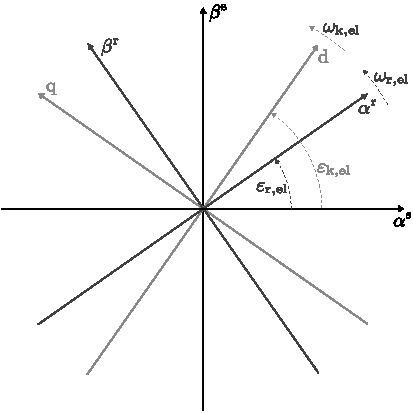
\includegraphics[width=0.85\textwidth]{fig/lec06/K_coordinates.pdf}
                \caption{Comparison of coordinate systems}
                \label{fig:K_coordinates}
            \end{figure}
        \end{column}
    \end{columns}
\end{frame}